\documentclass[final]{beamer}

\usepackage[scale=1.24]{beamerposter} % Use the beamerposter package for laying out the poster

\usepackage[utf8]{inputenc}
\usetheme{confposter} % Use the confposter theme supplied with this template

\setbeamercolor{block title}{fg=ngreen,bg=white} % Colors of the block titles
\setbeamercolor{block body}{fg=black,bg=white} % Colors of the body of blocks
\setbeamercolor{block alerted title}{fg=white,bg=dblue!70} % Colors of the highlighted block titles
\setbeamercolor{block alerted body}{fg=black,bg=dblue!10} % Colors of the body of highlighted blocks
% Many more colors are available for use in beamerthemeconfposter.sty

%-----------------------------------------------------------
% Define the column widths and overall poster size
% To set effective sepwid, onecolwid and twocolwid values, first choose how many columns you want and how much separation you want between columns
% In this template, the separation width chosen is 0.024 of the paper width and a 4-column layout
% onecolwid should therefore be (1-(# of columns+1)*sepwid)/# of columns e.g. (1-(4+1)*0.024)/4 = 0.22
% Set twocolwid to be (2*onecolwid)+sepwid = 0.464
% Set threecolwid to be (3*onecolwid)+2*sepwid = 0.708

\newlength{\sepwid}
\newlength{\onecolwid}
\newlength{\twocolwid}
\newlength{\threecolwid}
\setlength{\paperwidth}{36in} % A0 width: 46.8in
\setlength{\paperheight}{48in} % A0 height: 33.1in
\setlength{\sepwid}{0.024\paperwidth} % Separation width (white space) between columns
\setlength{\onecolwid}{0.22\paperwidth} % Width of one column
\setlength{\twocolwid}{0.464\paperwidth} % Width of two columns
\setlength{\threecolwid}{0.708\paperwidth} % Width of three columns
\setlength{\topmargin}{-0.5in} % Reduce the top margin size
%-----------------------------------------------------------

\usepackage{graphicx}  % Required for including images

\usepackage{booktabs} % Top and bottom rules for tables

%----------------------------------------------------------------------------------------
%	TITLE SECTION 
%----------------------------------------------------------------------------------------

\title{Sistema Simple de Pregunta y Respuesta en Español} % Poster title

\author{Cristóbal Donoso Oliva} % Author(s)

\institute{Ciencias de la Computación, Universidad de Concepción} % Institution(s)

%----------------------------------------------------------------------------------------

\begin{document}

\addtobeamertemplate{block end}{}{\vspace*{2ex}} % White space under blocks
\addtobeamertemplate{block alerted end}{}{\vspace*{2ex}} % White space under highlighted (alert) blocks

\setlength{\belowcaptionskip}{2ex} % White space under figures
\setlength\belowdisplayshortskip{2ex} % White space under equations

\begin{frame}[t] % The whole poster is enclosed in one beamer frame

\begin{columns}[t] % The whole poster consists of three major columns, the second of which is split into two columns twice - the [t] option aligns each column's content to the top

\begin{column}{\sepwid}\end{column} % Empty spacer column

\begin{column}{\onecolwid} % The first column

%----------------------------------------------------------------------------------------
%	OBJECTIVES
%----------------------------------------------------------------------------------------

\begin{alertblock}{Objetivos}

Los objetivos de este proyecto son
\begin{itemize}
\item Extraer información desde la web del tipo \textit{Quien} y \textit{Donde}
\item Entregar respuestas coherentes a consultas realizadas en lenguaje natural
\item Jerarquizar calidad de respuestas
\end{itemize}

\end{alertblock}

%----------------------------------------------------------------------------------------
%	INTRODUCTION
%----------------------------------------------------------------------------------------

\begin{block}{Introducción}
Internet es un gran banco de información la cual podemos capturar realizando lectura de cada uno de los documentos que allí se alojan. Estos documentos son páginas HTML cuyo contenido (texto plano) está delimitado por marcadores sintácticos propios del lenguaje.\textbf{Dada una consulta, es necesario utilizar métodos de recuperación y extracción de información con el objetivo de contestar cada pregunta}. A continuación, se muestra el desarrollo de un sistema simple de pregunta y respuesta para documentos virtuales en español. Las preguntas serán del tipo \textit{Quién} y \textit{Dónde}. Finalmente, se mostrarán los resultados obtenidos.\\
\begin{figure}
\centering
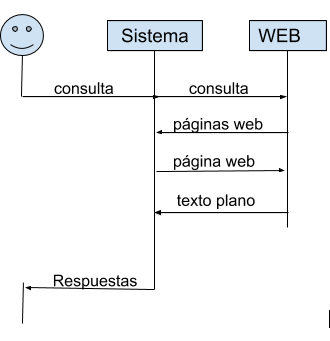
\includegraphics[scale=1.7]{img/diagrama.png} 
\caption{Diagrama de comunicación entre el usuario, el sistema y la web}
\end{figure}
\end{block}


%----------------------------------------------------------------------------------------

\end{column} % End of the first column

\begin{column}{\sepwid}\end{column} % Empty spacer column

\begin{column}{\twocolwid} % Begin a column which is two columns wide (column 2)

\begin{columns}[t,totalwidth=\twocolwid] % Split up the two columns wide column

\begin{column}{\onecolwid}\vspace{-.6in} % The first column within column 2 (column 2.1)

%----------------------------------------------------------------------------------------
%	MATERIALS
%----------------------------------------------------------------------------------------

\begin{block}{Ingresando la Pregunta}

El sistema cuenta con 7 partes: 
\begin{enumerate}
\item \textbf{Ingreso de la pregunta en lenguaje natural: }El usuario interactúa con el sistema escribiendo una consulta en español.
\item \textbf{Limpieza de la pregunta:} Una vez realizada la pregunta se procede a eliminar signos de interrogación. Luego se corta el Token que identifica el tipo de pregunta;\\por ej. 
\begin{center}
¿Quién es John Lennon? 
\end{center}
quedaría como 
\begin{center}
Quien es John Lennon 
\end{center}
y el identificador de pregunta sería \textbf{Quién}
\item \textbf{Búsqueda de páginas en la web:} Para realizar la búsqueda se añade un string en una url de google.
\begin{figure}
\centering
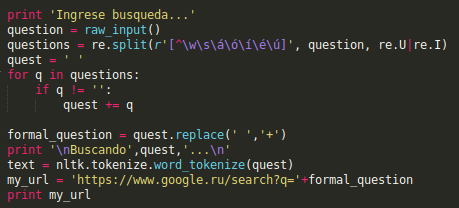
\includegraphics[scale=1.2]{img/google_link.png} 
\caption{Segmento de codigo donde se ingresa la pregunta a un link generico de google}
\end{figure}
\item \textbf{Extracción de respuestas:} Para extraer las respuesta se ingresa a cada una de las páginas utilizando los \textbf{request} de python. Luego con \textbf{BeautifulSoup} se extrae el texto plano (eliminando los identificadores sintácticos de HTML). Finalmente, utilizando \textbf{expresiones regulares}, extraemos las oraciones candidatas para ser respuesta.
\end{enumerate}

\end{block}

%----------------------------------------------------------------------------------------

\end{column} % End of column 2.1

\begin{column}{\onecolwid}\vspace{-.6in} % The second column within column 2 (column 2.2)

%----------------------------------------------------------------------------------------
%	METHODS
%----------------------------------------------------------------------------------------

\begin{block}{Entregando Respuesta}
\begin{enumerate}
\item \textbf{Clustering de respuestas:} Una vez extraída las oraciones realizamos una representación vectorial de cada una de las sentencias. Utilizamos \textbf{Agglomerative Clustering} \cite{day1984} con métrica de \textbf{distancia coseno}\cite{smith1997}. Los vectores ingresan como input en el modelo. Luego obtenemos los clusters; en este caso utilizamos \textbf{4 clusters}. Cada cluster representa un tipo de respuesta
\item \textbf{Selección de respuestas:} Seleccionamos la primera oración de cada cluster asumiendo que los primeros párrafos en un texto tienen más información global. Esto, porque la estructura de un corpus se torna más detallada a medida que avanzamos en los párrafos.
\item \textbf{Evaluación:} Para evaluar utilizamos Mean Reciprocal Rank. \begin{equation}
MRR = \frac{1}{Q}\sum_{i=1}^Q\frac{1}{rank_i}
\end{equation}
Donde $Q$ son la cantidad de palabras y $rank_i$ la cantidad de palabras que coinciden con la raiz. Por ej.
\begin{figure}
\centering
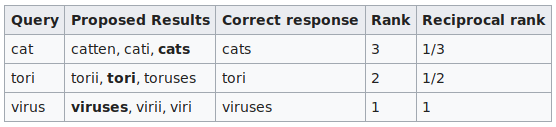
\includegraphics[scale=1]{img/tabla.png} 
\end{figure}
Dependiendo del tipo de pregunta (Quien o Donde) buscamos apariciones de palabras claves en un diccionario. Por ejemplo, si buscamos un lugar, entonces deberá aparecer el nombre de un país o ciudad.
\end{enumerate}

\end{block}

%----------------------------------------------------------------------------------------

\end{column} % End of column 2.2

\end{columns} % End of the split of column 2 - any content after this will now take up 2 columns width

%----------------------------------------------------------------------------------------
%	IMPORTANT RESULT
%----------------------------------------------------------------------------------------

\begin{alertblock}{Important Result}
\begin{figure}
\centering
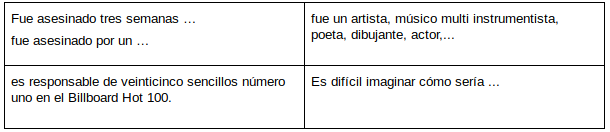
\includegraphics[scale=1.7]{img/clusters.png} 
\caption{4 cluster para la consulta "Quien es John Lennon"}
\end{figure}

\begin{center}
\begin{tabular}{|c|c|}
\hline 
\textbf{Pregunta} & \textbf{Mejor Respuesta} \\ 
\hline 
¿Quien fue Gabriela Mistral? & fue una poetisa, \\&diplomática y pedagoga chilena. \\ 
\hline 
¿Quien fue Alan Turing? & fue un pionero \\&de los campos de la computaci... \\ 
\hline 
¿Donde está Lota? & ubicada en la provincia de \\&Concepción, región del Biobío \\ 
\hline 
¿Donde está la Muralla China? & ubicada a menos \\&de 80 kilómetros de Pekín... \\ 
\hline 
\end{tabular} 
\end{center}
\end{alertblock} 

%----------------------------------------------------------------------------------------

\begin{columns}[t,totalwidth=\twocolwid] % Split up the two columns wide column again

\begin{column}{\onecolwid} % The first column within column 2 (column 2.1)

%----------------------------------------------------------------------------------------
%	MATHEMATICAL SECTION
%----------------------------------------------------------------------------------------



%----------------------------------------------------------------------------------------

\end{column} % End of column 2.1

\begin{column}{\onecolwid} % The second column within column 2 (column 2.2)



%----------------------------------------------------------------------------------------

\end{column} % End of column 2.2

\end{columns} % End of the split of column 2

\end{column} % End of the second column

\begin{column}{\sepwid}\end{column} % Empty spacer column

\begin{column}{\onecolwid} % The third column

%----------------------------------------------------------------------------------------
%	CONCLUSION
%----------------------------------------------------------------------------------------
\begin{block}{Resultados}
Para medir los resultados, se hizo uso solo del Rank. Lo anterior debido a que solo se contaba con un diccionario de palabras clave para cada pregunta. No se descarta la posibilidad de a futuro enriquecer estos diccionarios de manera de realizar el \textit{Mean Reciprocal Rank}. La figura 3 muestra los clusters generados y la figura 4 el ranking generado con las principales respuestas.
\begin{figure}
\centering
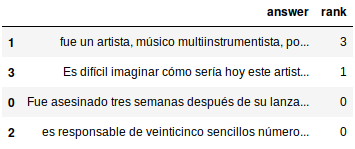
\includegraphics[scale=1.7]{img/rank.png} 
\caption{ranks asociados a las ocurrencias de palabras clave en la consulta \textit{Quien fue John Lennon}}
\end{figure}
\end{block}


\begin{block}{Conclusion}
Se ha realizado un sistema simple de pregunta y respuesta basado principalmente en expresiones regulares. El uso de Clusters permite separar las respuestas en grupos cuyo contenido es similar. A futuro, en vez de considerar clustering podríamos utilizar un modelo de clasificación de respuestas basado en Redes Neuronales Recurrentes.
\end{block}


%----------------------------------------------------------------------------------------
%	REFERENCES
%----------------------------------------------------------------------------------------

\begin{block}{References}

\nocite{*} % Insert publications even if they are not cited in the poster
\small{\bibliographystyle{unsrt}
\bibliography{sample}\vspace{0.75in}}

\end{block}

%----------------------------------------------------------------------------------------
%	CONTACT INFORMATION
%----------------------------------------------------------------------------------------

\setbeamercolor{block alerted title}{fg=black,bg=norange} % Change the alert block title colors
\setbeamercolor{block alerted body}{fg=black,bg=white} % Change the alert block body colors

\begin{alertblock}{Contact Information}

\begin{itemize}
\item Email: \href{mailto:cridonoso@inf.udec.cl}{cridonoso@inf.udec.cl}
\item Phone: +569 774 658 09
\end{itemize}

\end{alertblock}

\begin{center}
\begin{tabular}{ccc}

\includegraphics[width=0.4\linewidth]{./img/logo.png}  
\end{tabular}
\end{center}

%----------------------------------------------------------------------------------------

\end{column} % End of the third column

\end{columns} % End of all the columns in the poster

\end{frame} % End of the enclosing frame

\end{document}
